\PassOptionsToPackage{unicode=true}{hyperref} % options for packages loaded elsewhere
\PassOptionsToPackage{hyphens}{url}
%
\documentclass[12pt,]{article}
\usepackage{lmodern}
\usepackage{setspace}
\setstretch{2.0}
\usepackage{amssymb,amsmath}
\usepackage{ifxetex,ifluatex}
\usepackage{fixltx2e} % provides \textsubscript
\ifnum 0\ifxetex 1\fi\ifluatex 1\fi=0 % if pdftex
  \usepackage[T1]{fontenc}
  \usepackage[utf8]{inputenc}
  \usepackage{textcomp} % provides euro and other symbols
\else % if luatex or xelatex
  \usepackage{unicode-math}
  \defaultfontfeatures{Ligatures=TeX,Scale=MatchLowercase}
\fi
% use upquote if available, for straight quotes in verbatim environments
\IfFileExists{upquote.sty}{\usepackage{upquote}}{}
% use microtype if available
\IfFileExists{microtype.sty}{%
\usepackage[]{microtype}
\UseMicrotypeSet[protrusion]{basicmath} % disable protrusion for tt fonts
}{}
\IfFileExists{parskip.sty}{%
\usepackage{parskip}
}{% else
\setlength{\parindent}{0pt}
\setlength{\parskip}{6pt plus 2pt minus 1pt}
}
\usepackage{hyperref}
\hypersetup{
            pdfborder={0 0 0},
            breaklinks=true}
\urlstyle{same}  % don't use monospace font for urls
\usepackage[margin=1in]{geometry}
\usepackage{graphicx,grffile}
\makeatletter
\def\maxwidth{\ifdim\Gin@nat@width>\linewidth\linewidth\else\Gin@nat@width\fi}
\def\maxheight{\ifdim\Gin@nat@height>\textheight\textheight\else\Gin@nat@height\fi}
\makeatother
% Scale images if necessary, so that they will not overflow the page
% margins by default, and it is still possible to overwrite the defaults
% using explicit options in \includegraphics[width, height, ...]{}
\setkeys{Gin}{width=\maxwidth,height=\maxheight,keepaspectratio}
\setlength{\emergencystretch}{3em}  % prevent overfull lines
\providecommand{\tightlist}{%
  \setlength{\itemsep}{0pt}\setlength{\parskip}{0pt}}
\setcounter{secnumdepth}{0}
% Redefines (sub)paragraphs to behave more like sections
\ifx\paragraph\undefined\else
\let\oldparagraph\paragraph
\renewcommand{\paragraph}[1]{\oldparagraph{#1}\mbox{}}
\fi
\ifx\subparagraph\undefined\else
\let\oldsubparagraph\subparagraph
\renewcommand{\subparagraph}[1]{\oldsubparagraph{#1}\mbox{}}
\fi

% set default figure placement to htbp
\makeatletter
\def\fps@figure{htbp}
\makeatother


\date{}

\begin{document}

\hypertarget{introduction}{%
\section{Introduction}\label{introduction}}

\hypertarget{thermometry}{%
\subsection{Thermometry}\label{thermometry}}

Temperature is generally understood to be a measure of the average
kinetic energy contained in the atoms, electrons, and phonons (or other
quasiparticle excitations) which make up matter. Within the formalism of
statistical mechanics, we can compute compute the temperature within the
microcanonical ensemble as function of the total energy \(E\) and
information about the states of the system:
\[\frac{1}{T} = \frac{dS}{dE} = \frac{d}{dE} k \log W\] where \(W(E)dE\)
is the number of states with energy between \(E\) and \(E+dE\) and \(k\)
is Boltzmann's constant. This function, however, can only be computed
explicity for the simplest physical systems. In practice, if we want to
study the flow of heat through a system by measuring temperature, we
must find some other observable we can measure as a proxy.

In principle, we might want to find some system whose thermodynamic
equation of state depends on temperature and other quantities which are
all independant of temperature. Such a system is refered to as a primary
thermometer. For a simple example of such a thermometer, consider the
equation of state of an ideal gas: \[PV = NkT\] If we take a sample of
an ideal gas with a known number of molecules \(N\) in a known volume
\(V\), we can determine the temperature \(T\) by measuring its pressure
\(P\). Other examples of primary thermometers include measurements of
the speed of sound in a gas, measurements of the Johnson-Nyquist noise
in an electrical circuit, or measurements of blackbody radiation
{[}@Ekin2006{]}. These methods of measuring temperature are very useful
for accurately setting a temperature scale, but they have some serious
drawbacks as thermometers for use in other experiments. Most of them
require sensitive measurements of multiple physical observables, as well
as bulky and complicated experimental apparatus. If one wanted to
determine the thermal conductivity of a small crystal by measuring a
temperature gradient across its length, it would not be feasable to
connect the crystal to two independant samples of an ideal gas and
measure their pressures. Thus, the temperature standard set by these
methods must be transferred to a more convenient thermometer.

Such a device is known as a secondary thermometer. In this case, we
measure some observable as a function of temperature, which we determine
from some known standard. This can be a primary thermometer or another
secondary thermometer which has already been calibrated to sufficient
accuracy. In experimental condensed matter physics, by far the most
common types of secondary thermometers used are resistance thermometers
and thermocouples. Resistance thermometers simply measure the resistance
of some material as a proxy for temperature, either a metal such as
platinum (resistance increasing with higher temperature, or ``positive
temperature coefficent'') or a semiconductor, such as
zirconium--oxynitride (known by its trademarked name Cernox) or
ruthenium oxide (resistance decreasing with higher temperature, or
``negative temperature coefficent''). Such thermometers are convenient
since they can be made compact, they are commercially available, and
there are well--established protocols and instrumentation for measuring
resistance. There are a wide variety of resistance thermometers that
suit different temperature ranges and experimental conditions.
Thermocouples, which measure the temperature dependant thermopower
between two metals with differing carrier concentrations, can be even
more compact and are especially useful for making differential
measurements. However, they require measurments of DC voltages in the
microvolt range, and their sensitivy is reduced at low temperature. In
any case, both of these methods allow us to measure temperature without
considering the microscopic details of the system, only how accurately
it has been calibrated.

There are some experimental details which must be considered when using
a resistance thermometer. Many important experimental techniques in
condensed matter physics involve applying an intense magnetic field (up
to 45T for the current state-of-the-art DC magnets) to a sample of
interest. Resistance thermometers generally exhibit magnetoresistance,
the changing of their resistivity in a magnetic field. The most commonly
used resistance thermometers are selected to have as small a
magnetoresistnace as possible, but even Cernox thermometers display a
change of resistance of a few percent in magnetic fields up to 14T. If
one is not measuring any direct thermal property of a sample and can
safely assume that the sample is well thermalized with the cold finger,
one can simply mount a thermometer outside the region of intense
magnetic field. However, if you are measuring some thermal propety of a
material (such as heat capacity or thermal conductivity), there is no
getting around calibrating the thermometer as a function of temperature
and magnetic field (see figure \ref{cernox_fieldcal}). For semiconductor
thermometers such as Cernox, the magnetoresistance can vary quite a bit
from thermometer to thermometer, as they can have slightly different
doping levels. Additionally, the magnetoresistance depends in general on
the orientation of the thermometer with respect to the applied magnetic
field. Thus, the thermometer must either be calibrated in situ, or great
care must be taken to ensure that the thermometer's orientation is
preserved from experiment to experiment.

\begin{figure}
\centering
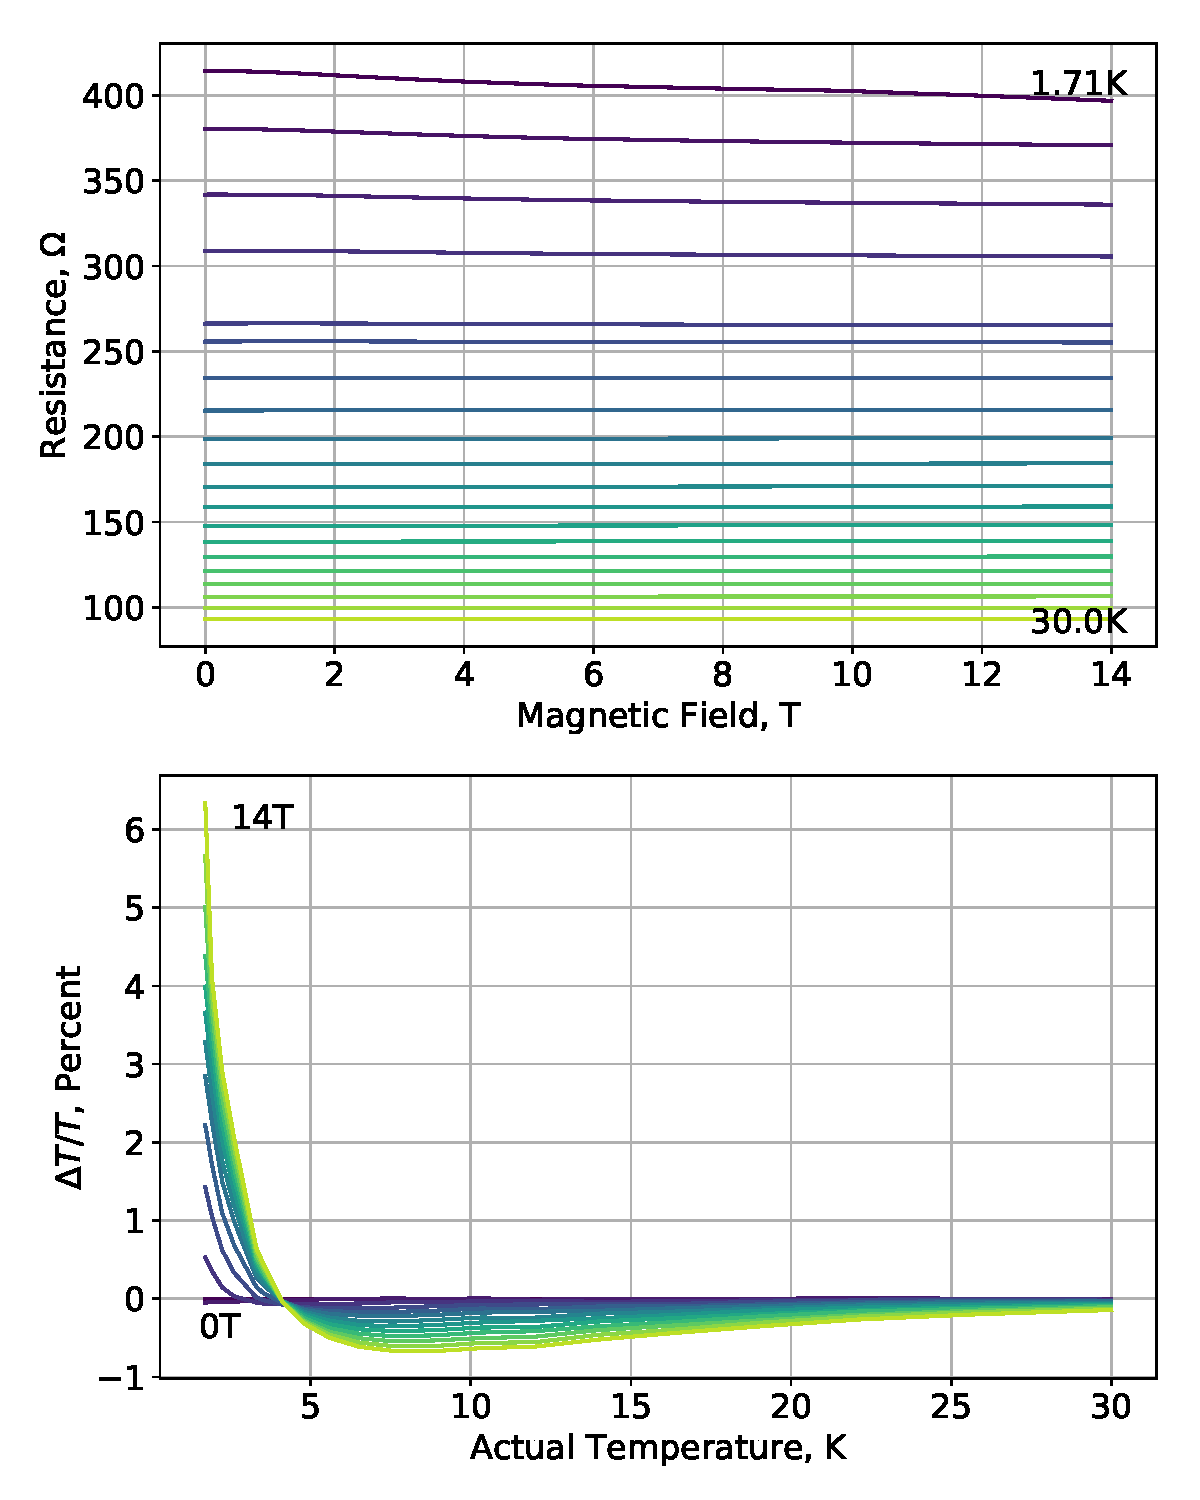
\includegraphics{figures/cal_cernox_1.pdf}
\caption{Example Cernox Field Calibration. Top: Magnetoresistance of a
Cernox thermometer. Bottom: Field calibration curves for the same
thermometer.
\((T_{\mathrm{apparent}} - T_{\mathrm{actual}})/T_{\mathrm{actual}}\) is
plotted versus the actual temperature. \label{cernox_fieldcal}}
\end{figure}

Regardless, there is a great deal of scientific value in thermal
measurments performed in strong magnetic fields. Heat capacity provides
a generic method for identifying phase transitions, and thermal
transport is sensitive to excitations in a solid which do not carry
charge and thus can't be studied with electrical transport methods.
Thus, it is our goal to develop new methods for accurately and precisely
measuring temperature in the presence of intense magnetic fields. The
scientific potential of these methods and the experimental techniques
they make possible will be underscored in the next section. For more
information about thermometry and its application in experimental
condensed matter physics, chapter 5 of {[}@Ekin2006{]} is an invaluable
reference.

\hypertarget{the-thermal-hall-effect}{%
\subsection{The Thermal Hall Effect}\label{the-thermal-hall-effect}}

The thermal Hall effect is the thermal analogue of the much more well
known (electrical) Hall effect. As the Hall effect can be understood as
generalizing the electrical conductivity \(\sigma\) to a tensor in Ohm's
law:
\[\mathbf{j} = \sigma \mathbf{E} \Rightarrow \begin{pmatrix} j_x \\ j_y
\end{pmatrix} = \begin{pmatrix} \sigma_{xx} & \sigma_{xy} \\ -\sigma_{xy} &
\sigma_{yy} \end{pmatrix} \begin{pmatrix} E_x \\ E_y \end{pmatrix} \]
The thermal Hall effect generalizes the thermal conductivity \(\kappa\)
to a tensor in Fourier's law:
\[\mathbf{q} = -\kappa \nabla u \Rightarrow \begin{pmatrix} q_x \\ q_y
\end{pmatrix} = -\begin{pmatrix} \kappa_{xx} & \kappa_{xy} \\ -\kappa_{xy} &
\kappa_{yy} \end{pmatrix} \begin{pmatrix} \partial_x u \\ \partial_y u
\end{pmatrix} \] where \(u\) is the temperature field. Before discussing
the origin of of the thermal Hall conductivity \(\kappa_{xy}\), we
should establish how heat flows through such a material. Let's assume we
have an isotropic material (i.e. \(\kappa_{xx} = \kappa_{xy}\)). The
conductivity tensor can be rewritten as
\[\begin{pmatrix} \kappa_{xx} & \kappa_{xy} \\ -\kappa_{xy} & \kappa_{xx}
\end{pmatrix} = \kappa_{xx} \begin{pmatrix} 1 & \kappa_{xy}/\kappa_{xx} \\
-\kappa_{xy}/\kappa_{xx} & 1 \end{pmatrix} = \kappa_{xx} \begin{pmatrix} 1 &
\tan \theta_H \\ -\tan \theta_H & 1 \end{pmatrix} \] where
\(\theta_H = \arctan \kappa_{xy}/\kappa_{xx}\) is the definition of the
thermal Hall angle. Writing down the Heat equation, and splitting the
conductivity into its symmetric and antisymmetric parts:
\begin{align*} -\nabla \cdot \mathbf{q} = c \rho \partial_t u = \nabla \cdot (\kappa \nabla u) &=
\nabla \cdot (\kappa_{xx}(\mathbb{I} + \kappa_{\mathrm{antisym}}) \nabla u) \\
&= \kappa_{xx}\nabla^2 u + \kappa_{xx}\nabla \cdot (\kappa_{\mathrm{antisym}}
\nabla u) \end{align*} where c is the heat capacity and \(\rho\) is the
mass density. Writing out the \(\kappa_\mathrm{antisym}\) term
explicitly:
\begin{align*}\begin{pmatrix} \partial_x & \partial_y \end{pmatrix} \begin{pmatrix} 0 & \tan
\theta_H \\ -\tan \theta_H & 0 \end{pmatrix} \begin{pmatrix} \partial_x u \\
\partial_y u \end{pmatrix} &= \begin{pmatrix} \partial_x & \partial_y
\end{pmatrix} \begin{pmatrix} \tan \theta_H \partial_x u \\ -\tan \theta_H
\partial_y u \end{pmatrix} \\ &= \tan \theta_H \partial_{xy} u - \tan \theta_H
\partial_{xy} u = 0\end{align*} Thus the equation reduces to the
isotropic heat equation,
\(c\rho \partial_t u = \kappa_{xx} \nabla^2 u\)! Thus, it might seem
like the thermal Hall conductivity would have no effect on the flow of
heat through the material. Indeed, when studying the heat equation, the
conductivity tensor \(\kappa\) is usually assumed to be symmetric.
However, if we impose the Neumann boundary condition
\(g = -\hat{n} \cdot \mathbf{q}\) for some known function \(g\), the
effect of the thermal Hall conductivity can be seen:
\begin{align*}-\hat{n} \cdot \mathbf{q} &= \hat{n} \cdot \kappa \nabla u \\
&= \kappa_{xx} \begin{pmatrix} n_x & n_y \end{pmatrix} \begin{pmatrix} 1 & \tan
\theta_H \\ -\tan \theta_H & 1 \end{pmatrix} \begin{pmatrix} \partial_x u \\
\partial_y u \end{pmatrix} \\ &= \kappa_{xx} \begin{pmatrix} n_x & n_y
\end{pmatrix} \begin{pmatrix} \partial_x u + \tan \theta_H \partial_y u \\
-\tan \theta_H \partial_x u + \partial_y u \end{pmatrix} \\ &= \kappa_{xx} n_x
(\partial_x u + \tan \theta_H \partial_y u) + \kappa_{xx} n_y (-\tan \theta_H
\partial_x u + \partial_y u)  \end{align*} Taking for example
\(\hat{n} = (1, 0)\) and \(g = 0\) (perfectly insulating boundary
conditions):
\[ 0 = - \hat{n} \cdot \mathbf{q} = \kappa_{xx} (\partial_x u + \tan \theta_H
\partial_y u) \Rightarrow \partial_x u = -\tan \theta_H \partial_y u\]
In general, the derivative normal to the boundary is specified in terms
of the transverse derivative and the thermal Hall angle.

In order to see what this kind of boundary condition does in practice,
we can simulate a material with a thermal Hall coefficent using the
finite element method. For simplicity, we will look first at steady
state solutions (i.e.~those with \(\partial_t u = 0\)). Thus we will
need to solve the elliptic partial differential equation
\(-\nabla \cdot (\kappa \nabla u) = 0\). We start by expressing this
equation in weak form by multiplying it by a test function \(v\) and
integrating over the function's domain \(\Omega\):
\[ -\nabla \cdot (\kappa \nabla u) = 0 \Rightarrow -\int_\Omega \nabla \cdot
(\kappa \nabla u) v dx = 0 \] The function \(u(x,y)\) is said to solve
the weak problem if this equation holds for all functions \(v(x,y)\),
where \(v(x, y) = 0\) anywhere we have specified \(u\) on the boundary
(i.e.~imposed Dirichlet boundary conditions). By integrating by parts,
this becomes:
\[ - \int_\Omega \nabla \cdot (\kappa \nabla u) v dx = \int_\Omega \kappa \nabla
u \cdot \nabla v dx - \int_{\partial \Omega} (\hat{n} \cdot \kappa\nabla u) v ds\]
where the second integral on the right hand side is over the boundary of
\(\Omega\). The second integral can be rewritten in terms of the Neumann
boundary condition:
\[ - \int_{\partial\Omega} (\hat{n} \cdot \kappa \nabla u) v ds =
\int_{\partial\Omega} g v ds\] and so we have cast the problem in a form
suitable for solving with the finite element method, in terms of the
bilinear form
\[ a(u, v) = \int_\Omega \kappa \nabla u \cdot \nabla v dx \] and the
linear form \[ L(v) = -\int_{\partial \Omega} g v ds \] as
\(a(u, v) = L(v)\). By discretizing the problem using standard methods
over a suitable mesh, the problem reduces to solving a linear system.
There are many references which go into detail on finite element
analysis, but I used {[}@LangtangenLogg2017{]} which covered the
specific Python library I used to run the following simulations.

\begin{figure}
\centering
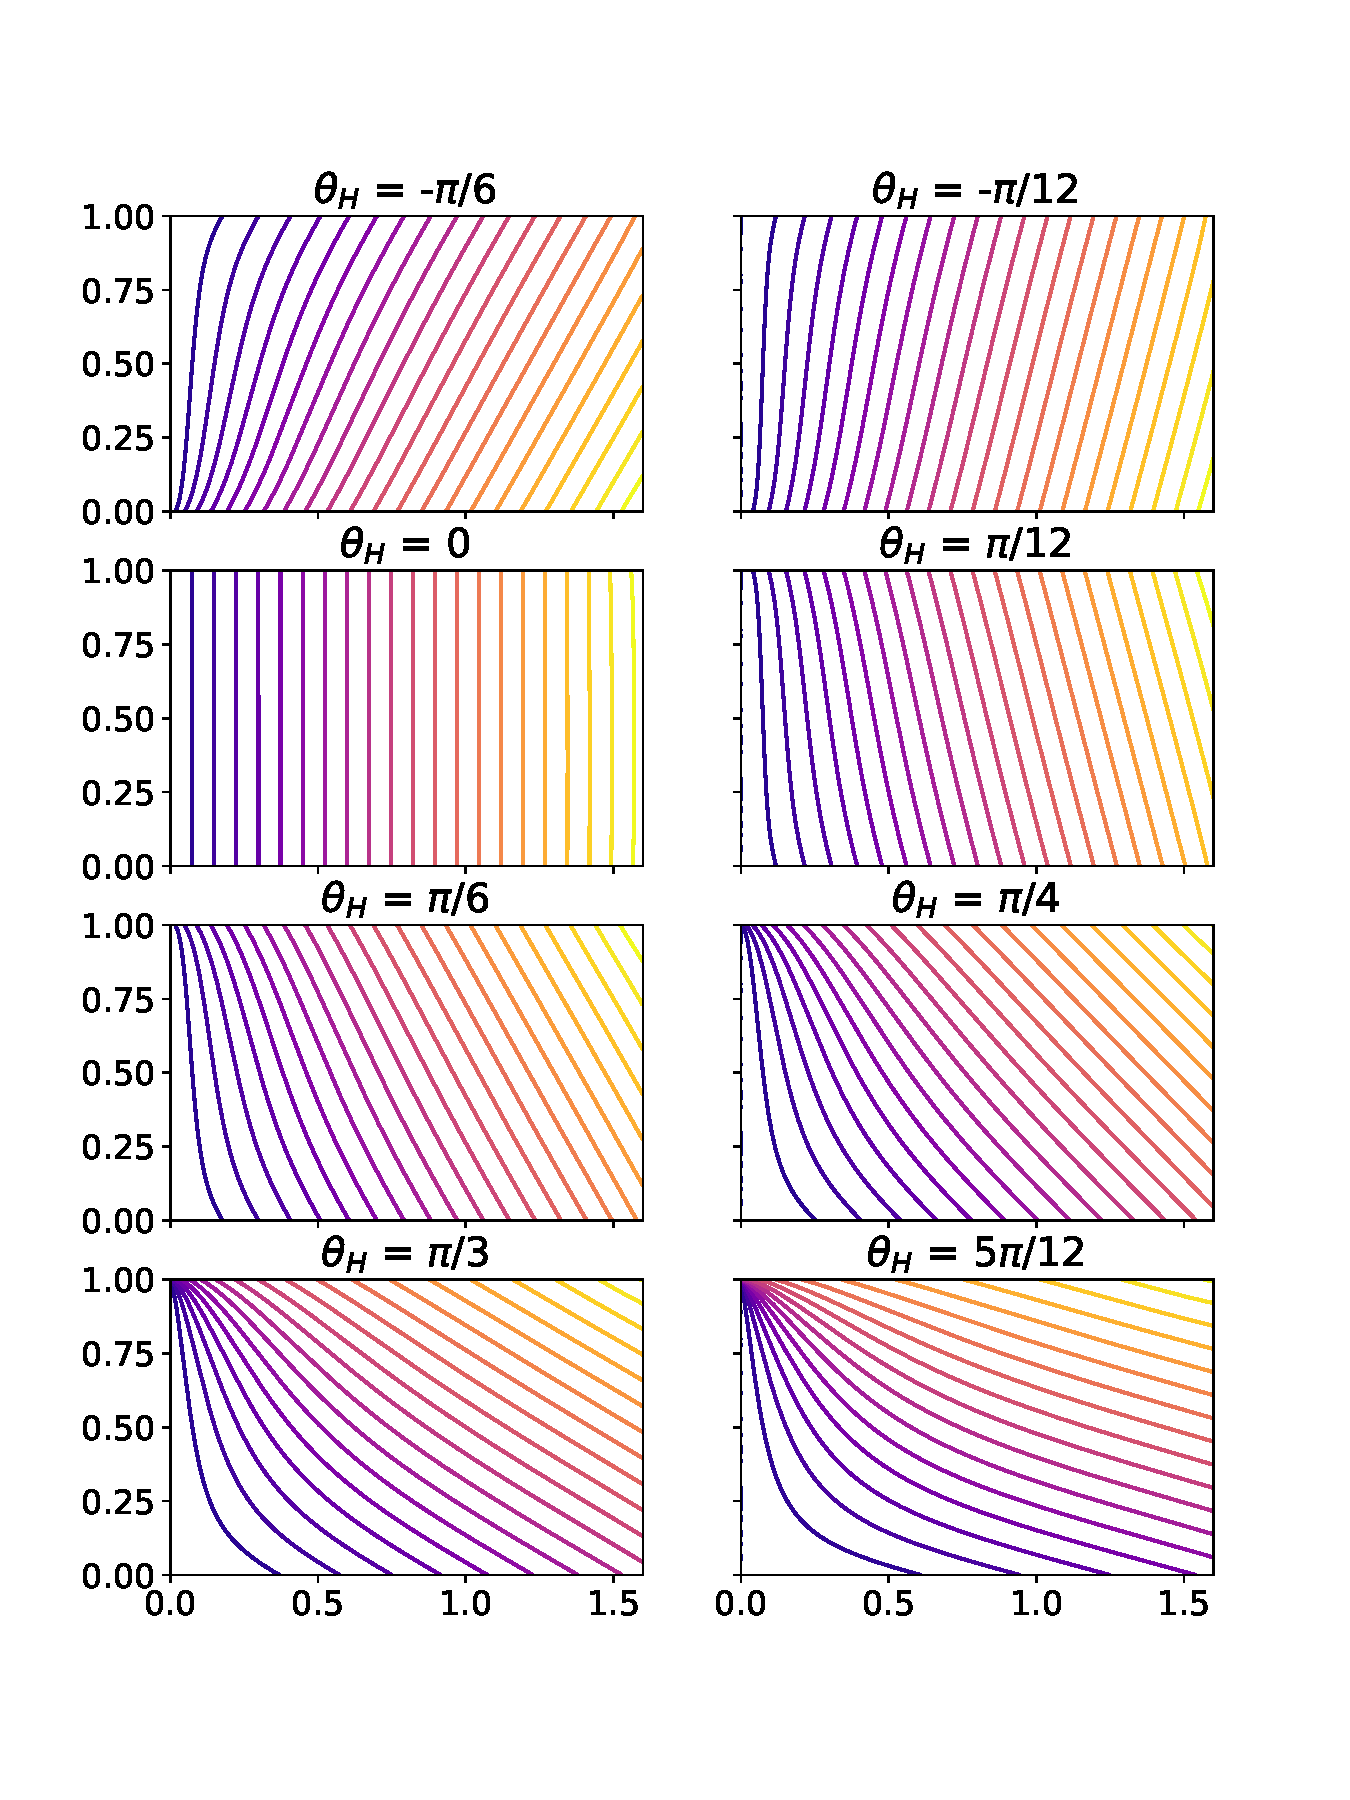
\includegraphics{figures/thall_isotherm.pdf}
\caption{Thermal Hall Isotherms. The left side of each simulation is
held to \(T=0\), the right has a heater with unit power, and the upper
and lower edges are insulating.\label{thall_iso}}
\end{figure}

\begin{figure}
\centering
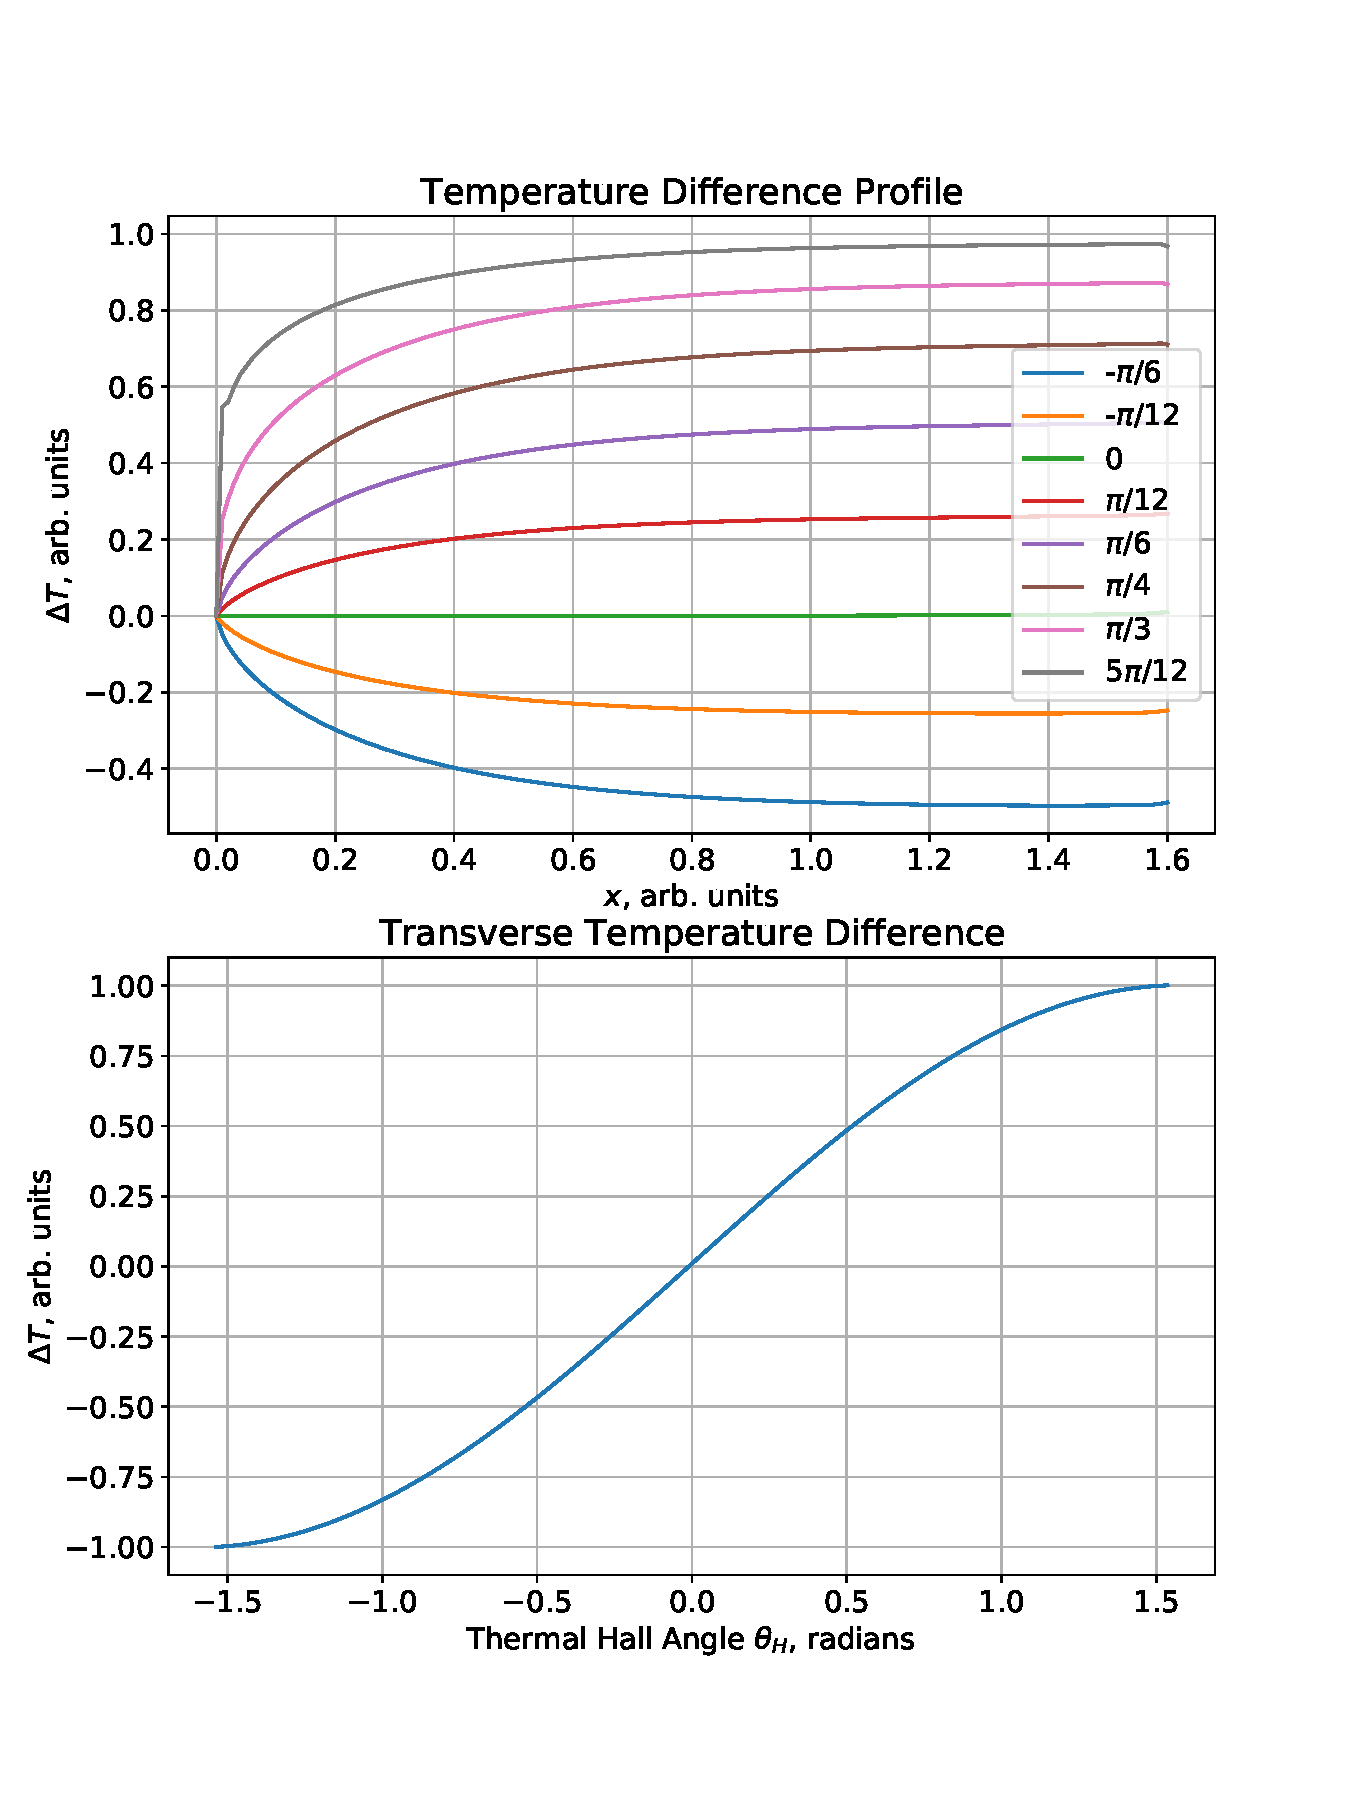
\includegraphics{figures/thall_profile.pdf}
\caption{Thermal Hall Temperature Profiles.\label{thall_prof}}
\end{figure}

\end{document}
